\documentclass[conference]{IEEEtran}
\IEEEoverridecommandlockouts
\usepackage{cite}
\usepackage[utf8]{inputenc}
\usepackage[english]{babel}
\usepackage{bookmark}
\usepackage[square,sort,comma,numbers]{natbib}
\usepackage{listings}
\usepackage{url}
\usepackage{wrapfig}
\usepackage{caption}
\usepackage{color}
\usepackage{enumitem}
\usepackage{graphicx}
\usepackage{float}
\usepackage{url}
\def\UrlBreaks{\do\/\do-}
\usepackage{breakurl}
\graphicspath{{images/}}
\usepackage{hyperref}


\def\BibTeX{{\rm B\kern-.05em{\sc i\kern-.025em b}\kern-.08em
T\kern-.1667em\lower.7ex\hbox{E}\kern-.125emX}}

\date{April 14, 2019}

\makeatletter
\let\thedate\@date


\definecolor{codegreen}{rgb}{0,0.6,0}
\definecolor{codegray}{rgb}{0.5,0.5,0.5}
\definecolor{codepurple}{rgb}{0.58,0,0.82}
\definecolor{backcolour}{rgb}{0.95,0.95,0.92}

\lstdefinestyle{mystyle}{
    backgroundcolor=\color{backcolour},   
    commentstyle=\color{codegreen},
    keywordstyle=\color{magenta},
    numberstyle=\tiny\color{codegray},
    stringstyle=\color{codepurple},
    basicstyle=\scriptsize,
    breakatwhitespace=false,         
    breaklines=true,                 
    captionpos=b,                    
    keepspaces=true,                 
    numbers=left,                    
    numbersep=5pt,                  
    showspaces=false,                
    showstringspaces=false,
    showtabs=false,                  
    tabsize=2
}
    
\lstset{style=mystyle}

\begin{document} 
    \title{
        Project CTE Document for Midterm 2\\[0.2cm]
        \large ELE494-08\\
        \large \thedate
    }

    \author{
        \IEEEauthorblockN{Nasir Khalid}
        \IEEEauthorblockA{B00065082\\}
    }

    \maketitle

    \section{Goal Statement}

    We aim to develop an autonomous robot that can survey a given location and return the point of
    maximum light intensity within that location. As it moves it will be sending back data in real
    time to a web browser on a phone/computer. 

    \section{Objective}

    The robot will be given a predefined map and it will be given it's starting position within that map.
    After this it will begin planning the path it will take around this location and during it's journey it
    will read the light intensity of the points. As it does this it will be sending back data of it's current
    position on the map \& the light intensity at its position. All of this will be visualized so we can watch
    it in real time. Once it's journey is complete it will go back and remain idle at the point which it determined
    to be the brightest.
 
    \section{Hardware}

    The main components of this device are:

    \begin{enumerate}
        \item Robot Body
        \begin{figure}[H]
        \centering
        \captionsetup{justification=centering}
        \centering
            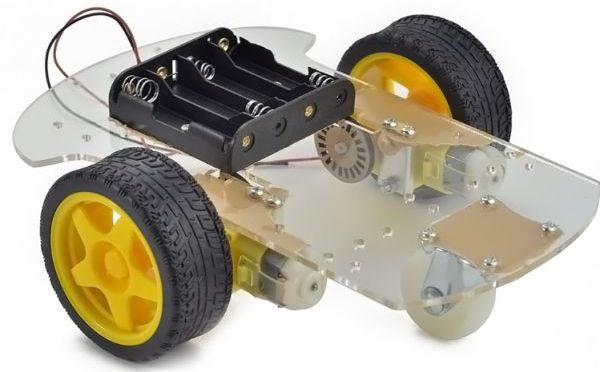
\includegraphics[width=0.15\textwidth]{chasis.jpg}
            \caption{Chassis, wheels and motors of robot \cite{Chassis}}
        \end{figure}

        \item NodeMCU Microcontroller
        \begin{figure}[H]
        \centering
        \captionsetup{justification=centering}
        \centering
            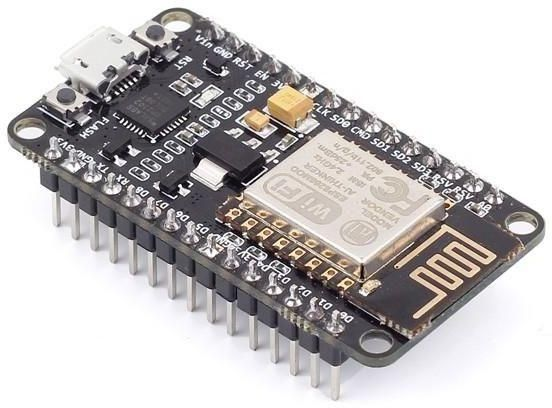
\includegraphics[width=0.15\textwidth]{Microcontroller.jpg}
            \caption{ESP8266 based NODEMCU microcontroller \cite{Microcontroller}}
        \end{figure}

        \item H-Bridge
        \begin{figure}[H]
        \centering
        \captionsetup{justification=centering}
        \centering
            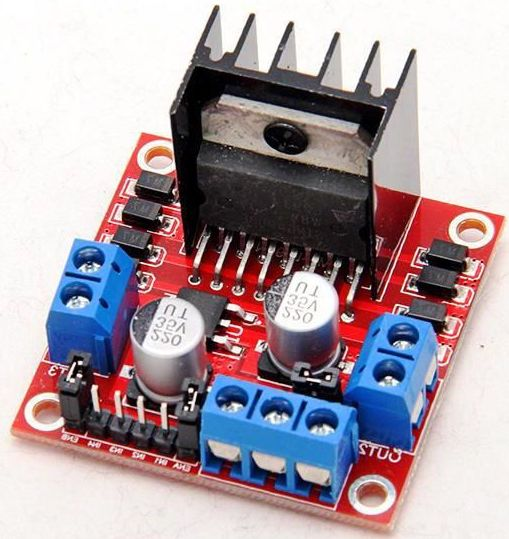
\includegraphics[width=0.15\textwidth]{hbrridge.jpg}
            \caption{Dual H-Bridge motor controllers \cite{HB}}
        \end{figure}

        \item Speed Encoders
        \begin{figure}[H]
        \centering
        \captionsetup{justification=centering}
        \centering
            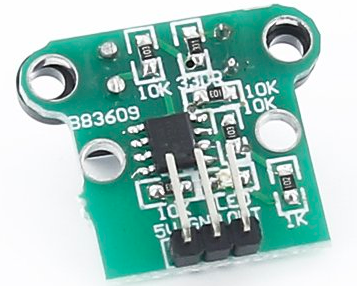
\includegraphics[width=0.15\textwidth]{enc.png}
            \caption{HC-020K Speed Measuring Module \cite{enc}}
        \end{figure}

        \item Power Bank
        \begin{figure}[H]
        \centering
        \captionsetup{justification=centering}
        \centering
            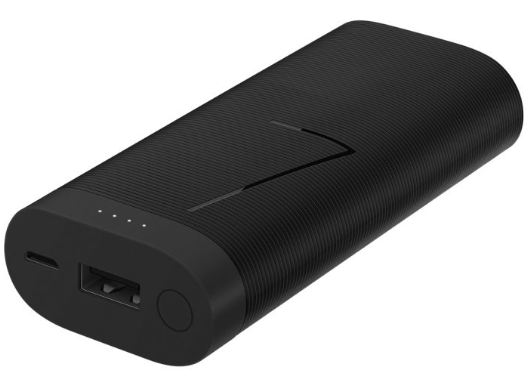
\includegraphics[width=0.15\textwidth]{pb.png}
            \caption{Huawei 6700 mAH power bank \cite{pb}}
        \end{figure}

    \end{enumerate}

    The final components (6 and 7) we currently do not have but we plan to purchase them soon\\

    \begin{enumerate}[resume]

        \item Accelerometer
        \begin{figure}[H]
        \centering
        \captionsetup{justification=centering}
        \centering
            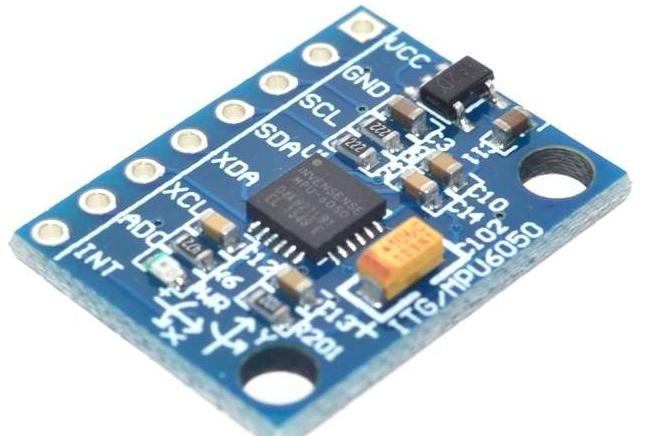
\includegraphics[width=0.15\textwidth]{g.png}
            \caption{MPU6050 3 axis accelerometer/gyroscope \cite{g}}
        \end{figure}

        \item Light Dependent Resistor
        \begin{figure}[H]
        \centering
        \captionsetup{justification=centering}
        \centering
            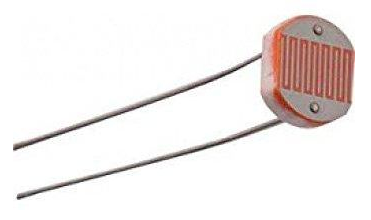
\includegraphics[width=0.15\textwidth]{ldr.png}
            \caption{Photoresistor LDR CDS 5mm \cite{LDR}}
        \end{figure}

    \end{enumerate}
    
    \section{Plan of Action}

    \subsection{Individual Tests}

    We will begin by testing each sensor independently with the NODEMCU microcontroller and
    try to get their output to display on a web server that can be accessed by phone or mobile.
    This will help us ensure that each sensor works properly and that we are using the right
    functions to interface with them

    \subsection{Joint Tests}

    After the individual tests are complete we will wire all the components together on a
    breadboard and create a circuit diagram for the entire system. Through this test it will
    be clear that all the components are working together and during this time we will be writing
    the preliminary code for the system.

    \subsection{Assembly}

    Now we will assemble all the components on to the chassis of the robot and execute the same
    preliminary code written in the previous section to ensure that it is operational and that wiring
    was correctly done.

    \subsection{Early Implementation}

    Now that the robot is ready we will modify it's code heavily to implement the following:

    \begin{enumerate}
        \item Path planning based on a given map
        \item Kalman filtration for position
        \item Visualization of position
        \item Real time graphing of filtered and unfiltered data
        \item All movement and robot control functions
    \end{enumerate}

    \subsection{Final Implementation}

    After the early testing stage we will implement the final part of the robot which is all the logic
    and control to identify the brightest spot in a given location.
    
    \section{Results}

    \subsection{Current Results}

    As of now we have individually tested and jointly tested the sensors we already own
    Currently the testing includes interfacing the microcontroller with the encoder, h-bridge,
    and activating the webserver to see data in real time. Shown below is the current set up
    for joint testing and also the results we obtained from the web server based on testing
    of the encoders.\\

    \begin{figure}[H]
        \centering
        \captionsetup{justification=centering}
        \centering
        \includegraphics[width=0.5\textwidth]{im.png}
        \caption{Joint Testing setup}
    \end{figure}

    \begin{figure}[H]
        \centering
        \captionsetup{justification=centering}
        \centering
        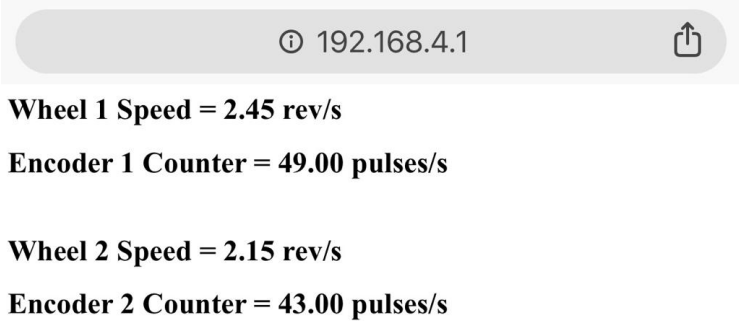
\includegraphics[width=0.4\textwidth]{t2.png}
        \caption{Encoder results from initial joint setup}
    \end{figure}

    Initial results from the encoders show a discrepancy between wheel 1 and wheel 2 even though
    the same speed is expected from both. This shows that we need to perform some filtration on
    the encoder results and also highlights the importance of the accelerometer because without it
    we would be unable to do position estimation. 

    \subsection{Future Results}

    For the next few stages we expect the robot to display the position more accurately and also
    provide a live graph highlighting the filtered and unfiltered data so we can see the effects.
    If possible we would also like to visualize certain other state variables and create a model
    of the robot that moves in realtime within a 3D map
    
    \section{Team Member Roles}

    Up until this stage of the project me and Youssef worked interchange on programming the robot
    and testing the various sensors. However the circuitry was handled by Youssef and the code for
    the web server and visualization was handled by me. Through this we understood our strong points
    and form now onwards we are dividing specific sections of the project between the two of us.\\

    Both of us will work on programming the microcontroller, interfacing with the sensors and code
    for filtering data.\\

    Youssef will work on circuitry and specific logic needed to convert sensor data to understandable
    readings\\

    I will work on visualization and robot functions for movement and control

    \begin{figure}[H]
        \centering
        \captionsetup{justification=centering}
        \centering
        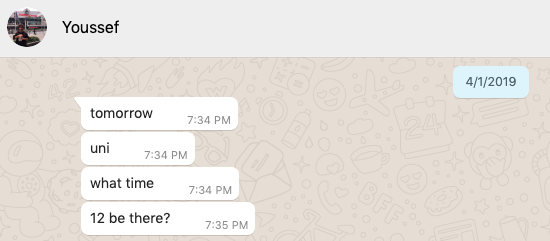
\includegraphics[width=0.4\textwidth]{m1.png}
        \caption{Planning first meeting during spring break}
    \end{figure}

    \begin{figure}[H]
        \centering
        \captionsetup{justification=centering}
        \centering
        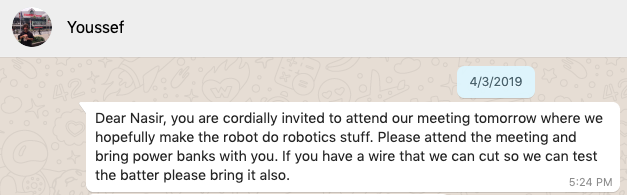
\includegraphics[width=0.4\textwidth]{m2.png}
        \caption{Planning second meeting during spring break}
    \end{figure}

    \section{Current State}

    \subsection{Hardware}

    Currently the circuit is system is set up for joint testing as shown in Figure 8. The hardware is
    connected and are using a lab bench top power supply for testing. The set up is currently in the
    microwave lab and can be accessed at any time if one has lab access.
    
    \subsection{Software}

    All software is listed in the appendix. A.3 and A.4 were written by Youssef. A.5 was written by me.
    The remaining code was written by both of us.

    \newpage
    \bibliographystyle{IEEEtran}
    \bibliography{proposal}
    \appendix

\begin{lstlisting}[language=C++, caption=Initializaion Code]
#include <ESP8266WiFi.h>
#include <WiFiClient.h>
#include <ESP8266WebServer.h>

//Pin Definitions

#define ENCODER1 5 //[D1]
#define ENCODER2 12 //[D6]

#define EN1  4  //[D2] 44 ON BREADBOARD
#define IN1  3  //[rx]
#define IN2  1 //[tx]

#define EN2  14 //[D5] 35 on BREADBOARD
#define IN3  16 //[D0] 43 ON BREADBOARD
#define IN4  13 //[D7] 42 ON BREADBOARD 


const char* ssid = "Robot";

float count1;
float count2;
float rev1;
float rev2;
float rev1_f;
float rev2_f;
String message;

ESP8266WebServer server(80);\end{lstlisting}

\begin{lstlisting}[language=C++, caption=Setup Function]
void setup() {
  delay(1000);
  
  //Defining PIN directions
  
  pinMode(EN1, OUTPUT);
  pinMode(IN1, OUTPUT);
  pinMode(IN2, OUTPUT);
  pinMode(EN2, OUTPUT);
  pinMode(IN3, OUTPUT);
  pinMode(IN4, OUTPUT);
  
  delay(1000);
  WiFi.softAP(ssid);

  IPAddress myIP = WiFi.softAPIP();
  
  analogWrite(EN1, 512); 
  analogWrite(EN2, 512);
  digitalWrite(IN1, HIGH);
  digitalWrite(IN2, LOW);
  digitalWrite(IN3, LOW);
  digitalWrite(IN4, HIGH);
  
  server.on("/", handleRoot);
  server.begin();

  pinMode(ENCODER1, INPUT);
  pinMode(ENCODER2, INPUT);

  attachInterrupt(
      digitalPinToInterrupt(ENCODER1),
      High_Callback,
      RISING
    );
  attachInterrupt(
      digitalPinToInterrupt(ENCODER2),
      Low_Callback,
      RISING
    );
}\end{lstlisting}

\begin{lstlisting}[language=C++, caption=Encoder Counter Math]
void loop(){
    rev1 = 0;
    rev2 = 0;
    for(int j=1; j<11;j++){
        count1 = 0;
        count2 = 0;
        delay(100);
        
        rev1 += count1 / 20; //number of revolutions
        rev2 += count2 / 20; //number of revolutions
        
    }
    rev1_f = rev1;
    rev2_f = rev2;
    server.handleClient();
    delay(100);
}\end{lstlisting}

\begin{lstlisting}[language=C++, caption=Callback Functions for Encoders]
void High_Callback(){
  count1 += 1;
}
void Low_Callback(){
  count2 += 1;
}\end{lstlisting} 

\begin{lstlisting}[language=C++, caption=Server Code to display Encoder Data]
void handleRoot(){
    message = "<h1>Wheel 1 Speed = ";
    message += String(rev1_f);
    message += " rev/s";
    message +=  "</h1>";

    message += "<h1>Encoder 1 Counter = ";
    message += String(count1);
    message += " pulses/s";
    message +=  "</h1>";
    message +=  "<br>";

    message += "<h1>Wheel 2 Speed = ";
    message += String(rev2_f);
    message += " rev/s";
    message +=  "</h1>";

    message += "<h1>Encoder 2 Counter = ";
    message += String(count2);
    message += " pulses/s";
    message +=  "</h1>";
    message +=  "<br>";

    server.send(200, "text/html",  message);}\end{lstlisting}
\end{document}